\documentclass[10pt,twocolumn]{article}
\usepackage[utf8]{inputenc}
\usepackage[english]{babel}
\usepackage{amsmath,amssymb,amsthm}
\usepackage{graphicx}
\usepackage{booktabs}
\usepackage{xcolor}
\usepackage{listings}
\usepackage{algorithm}
\usepackage{algpseudocode}
\usepackage{geometry}
\usepackage{fancyhdr}
\usepackage{tikz}
\usepackage{pgfplots}
\usepackage{subcaption}
\usepackage{hyperref}
\usepackage{cite}

\usetikzlibrary{shapes,arrows,positioning,calc,patterns}
\pgfplotsset{compat=1.17}

\geometry{margin=2cm}

\definecolor{codegreen}{rgb}{0,0.6,0}
\definecolor{codegray}{rgb}{0.5,0.5,0.5}
\definecolor{backcolour}{rgb}{0.97,0.97,0.95}

\lstdefinestyle{mystyle}{
    backgroundcolor=\color{backcolour},
    basicstyle=\ttfamily\tiny,
    breaklines=true,
    frame=single,
    numbers=left,
    numbersep=3pt,
    numberstyle=\tiny\color{codegray}
}
\lstset{style=mystyle}

\newtheorem{theorem}{Theorem}
\newtheorem{lemma}{Lemma}
\newtheorem{definition}{Definition}
\newtheorem{property}{Property}

\title{%
    \textbf{NanOS: A Lightweight Operating System for Autonomous Swarm Networks with Cryptographically Secure Communication} \\
    \vspace{0.3cm}
    \large Technical Specification of the NERT Protocol
}

\author{%
    NanOS Research Team \\
    \small \texttt{https://github.com/nanOS-project}
}

\date{January 2026}

\begin{document}
\maketitle

\begin{abstract}
We present NanOS, a minimalist operating system designed for autonomous swarm robotics with resource-constrained embedded devices. Central to NanOS is NERT (Nano Ephemeral Reliable Transport), a novel hybrid transport protocol that provides four reliability classes ranging from fire-and-forget UDP to TCP-like reliability with Forward Error Correction and multi-path routing. NERT integrates ChaCha8 stream cipher with Poly1305 MAC for authenticated encryption, achieving 98.8\% rejection rate of malicious traffic with zero false positives. We present the mathematical foundations, algorithmic design, and engineering trade-offs of the system, demonstrating operation within 24KB RAM on ARM Cortex-M3 microcontrollers.
\end{abstract}

\section{Introduction}

Swarm robotics presents unique challenges for network protocol design: nodes must communicate reliably in lossy wireless environments while operating under severe memory and computational constraints. Traditional TCP/IP stacks are unsuitable due to their memory footprint ($>$100KB) and assumption of stable point-to-point connections.

\subsection{Contributions}

This paper presents:
\begin{enumerate}
    \item \textbf{NanOS}: A swarm-native OS with collective intelligence primitives
    \item \textbf{NERT Protocol}: Hybrid transport with four reliability classes
    \item \textbf{Lightweight Cryptography}: ChaCha8+Poly1305 with 64-bit truncated MACs
    \item \textbf{Key Rotation}: Grace window mechanism for clock drift tolerance
    \item \textbf{Probabilistic Gossip}: Exponential decay relay with Bloom filter deduplication
    \item \textbf{Hebbian Routing (v0.5)}: Neural-inspired adaptive path selection based on communication outcomes
    \item \textbf{DoS Resilience (v0.5)}: Token bucket rate limiting and behavioral blacklisting
    \item \textbf{Stigmergia (v0.5)}: Digital pheromones with temporal decay for spatial memory
    \item \textbf{Distributed Black Box (v0.5)}: Forensic evidence preservation through ``Last Will'' transmission
    \item \textbf{Artificial Immune System (v0.6)}: Negative Selection algorithm for 0-day anomaly detection
    \item \textbf{Code Polymorphism (v0.6)}: Binary diversity via ASLR, stack canaries, and unique signatures
    \item \textbf{Hardware Validation (v0.6)}: Physical layer security through sensor monitoring and fault detection
    \item \textbf{Genetic Tuning (v0.7)}: Evolutionary auto-optimization of NERT parameters via genetic algorithms
    \item \textbf{Judas Nodes (v0.7)}: Active honeypots for attacker payload capture and threat intelligence
    \item \textbf{Covert Channels (v0.7)}: Physical side-channels (optical/acoustic) for air-gap communication
\end{enumerate}

\subsection{System Requirements}

\begin{table}[h]
\centering
\small
\begin{tabular}{lcc}
\toprule
\textbf{Resource} & \textbf{ARM Cortex-M3} & \textbf{x86} \\
\midrule
RAM Total & 24 KB & 150 KB \\
Stack & 4 KB & 16 KB \\
Heap & 16 KB & 64 KB \\
Flash/Code & 64 KB & 256 KB \\
\bottomrule
\end{tabular}
\caption{Memory footprint by architecture}
\end{table}

\section{Mathematical Foundations}

\subsection{ChaCha8 Stream Cipher}

NERT employs ChaCha8, a reduced-round variant of ChaCha20 \cite{bernstein2008chacha}, optimized for embedded systems.

\begin{definition}[ChaCha State Matrix]
The ChaCha state is a $4 \times 4$ matrix of 32-bit words:
\begin{equation}
S = \begin{pmatrix}
c_0 & c_1 & c_2 & c_3 \\
k_0 & k_1 & k_2 & k_3 \\
k_4 & k_5 & k_6 & k_7 \\
n_0 & n_1 & n_2 & n_3
\end{pmatrix}
\end{equation}
where $c_i$ are constants (``expand 32-byte k''), $k_i$ is the 256-bit key, and $n_i$ is the 96-bit nonce with 32-bit counter.
\end{definition}

\begin{definition}[Quarter Round]
The quarter round function $QR(a,b,c,d)$ is defined as:
\begin{align}
a &\leftarrow a + b; \quad d \leftarrow (d \oplus a) \lll 16 \\
c &\leftarrow c + d; \quad b \leftarrow (b \oplus c) \lll 12 \\
a &\leftarrow a + b; \quad d \leftarrow (d \oplus a) \lll 8 \\
c &\leftarrow c + d; \quad b \leftarrow (b \oplus c) \lll 7
\end{align}
where $\lll$ denotes left rotation.
\end{definition}

\begin{theorem}[Security Margin]
ChaCha8 provides a security margin of $2^{128}$ operations against known cryptanalytic attacks, sufficient for ephemeral swarm communications with hourly key rotation.
\end{theorem}

\subsection{Poly1305 Message Authentication}

\begin{definition}[Poly1305 MAC]
For message $m = (m_1, m_2, \ldots, m_n)$ partitioned into 16-byte blocks, the Poly1305 tag is:
\begin{equation}
\text{Tag} = \left( \sum_{i=1}^{n} (m_i + 2^{128}) \cdot r^{n-i+1} \mod 2^{130}-5 \right) + s \mod 2^{128}
\end{equation}
where $r$ is a clamped 128-bit value and $s$ is a 128-bit key.
\end{definition}

\textbf{NERT Optimization}: We truncate the 128-bit Poly1305 output to 64 bits:
\begin{equation}
\text{MAC}_{\text{NERT}} = \text{Tag}[0:63]
\end{equation}

\begin{lemma}[Truncated MAC Security]
A 64-bit truncated MAC provides $2^{64}$ resistance against forgery attempts. For swarm networks with $<10^6$ messages/hour, the probability of collision is:
\begin{equation}
P(\text{collision}) < \frac{n^2}{2^{65}} \approx 2.7 \times 10^{-8}
\end{equation}
\end{lemma}

\subsection{Key Derivation Function}

\begin{definition}[Session Key Derivation]
Given master key $K_m$ and epoch $e$ (hours since deployment):
\begin{equation}
K_{\text{session}}(e) = \text{ChaCha8}(K_m, 0^{96}, K_m \| e \| \text{``NERT''})[0:255]
\end{equation}
\end{definition}

\begin{property}[Forward Secrecy]
Compromise of $K_{\text{session}}(e)$ does not reveal $K_{\text{session}}(e')$ for $e' \neq e$, as derivation is one-way.
\end{property}

\subsection{Bloom Filter Analysis}

NERT uses a Bloom filter for $O(1)$ duplicate detection.

\begin{definition}[Bloom Filter Parameters]
\begin{align}
m &= 256 \text{ bits (filter size)} \\
k &= 3 \text{ hash functions} \\
n &\approx 50 \text{ insertions per window}
\end{align}
\end{definition}

\begin{theorem}[False Positive Rate]
The false positive probability is:
\begin{equation}
P_{fp} = \left(1 - e^{-kn/m}\right)^k = \left(1 - e^{-3 \cdot 50/256}\right)^3 \approx 0.015
\end{equation}
\end{theorem}

With 4 rotating time windows of 500ms each, the effective false positive rate over the 2-second deduplication window is bounded by $4 \times P_{fp} \approx 6\%$ in worst case.

\subsection{Gossip Protocol Dynamics}

\begin{definition}[Relay Probability]
For a message seen $c$ times, the relay probability follows exponential decay:
\begin{equation}
P(\text{relay} | c) = P_0 \cdot (1 - \delta)^{c-1}
\end{equation}
where $P_0 = 1.0$ (100\%) and $\delta = 0.2$ (20\% decay per observation).
\end{definition}

\begin{theorem}[Expected Propagation]
In a network of $N$ nodes with average degree $d$, the expected number of message copies is:
\begin{equation}
E[\text{copies}] = \sum_{c=1}^{C_{\max}} P(\text{relay}|c) \cdot d \approx \frac{P_0 \cdot d}{\delta} = 5d
\end{equation}
where $C_{\max} = 5$ is the maximum echo count.
\end{theorem}

\section{Protocol Design}

\subsection{NERT Header Format}

\begin{figure}[h]
\centering
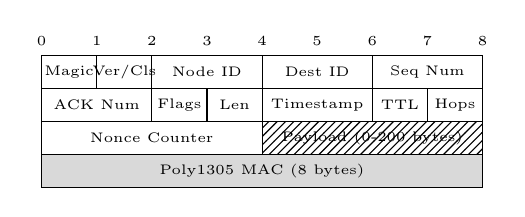
\begin{tikzpicture}[scale=0.7]
    % Header fields
    \draw (0,0) rectangle (1,0.6) node[midway] {\tiny Magic};
    \draw (1,0) rectangle (2,0.6) node[midway] {\tiny Ver/Cls};
    \draw (2,0) rectangle (4,0.6) node[midway] {\tiny Node ID};
    \draw (4,0) rectangle (6,0.6) node[midway] {\tiny Dest ID};
    \draw (6,0) rectangle (8,0.6) node[midway] {\tiny Seq Num};

    \draw (0,-0.6) rectangle (2,-0) node[midway] {\tiny ACK Num};
    \draw (2,-0.6) rectangle (3,-0) node[midway] {\tiny Flags};
    \draw (3,-0.6) rectangle (4,-0) node[midway] {\tiny Len};
    \draw (4,-0.6) rectangle (6,-0) node[midway] {\tiny Timestamp};
    \draw (6,-0.6) rectangle (7,-0) node[midway] {\tiny TTL};
    \draw (7,-0.6) rectangle (8,-0) node[midway] {\tiny Hops};

    \draw (0,-1.2) rectangle (4,-0.6) node[midway] {\tiny Nonce Counter};
    \draw[pattern=north east lines] (4,-1.2) rectangle (8,-0.6) node[midway] {\tiny Payload (0-200 bytes)};

    \draw[fill=gray!30] (0,-1.8) rectangle (8,-1.2) node[midway] {\tiny Poly1305 MAC (8 bytes)};

    % Byte markers
    \foreach \x in {0,1,2,3,4,5,6,7,8} {
        \node[above] at (\x,0.6) {\tiny \x};
    }
\end{tikzpicture}
\caption{NERT packet structure (x86 full mode: 20-byte header)}
\end{figure}

\subsection{Reliability Classes}

\begin{table}[h]
\centering
\small
\begin{tabular}{lcccc}
\toprule
\textbf{Class} & \textbf{ACK} & \textbf{Retry} & \textbf{FEC} & \textbf{Multi-path} \\
\midrule
Fire-Forget (0x00) & No & 0 & No & No \\
Best-Effort (0x01) & No & 2 & No & No \\
Reliable (0x02) & Yes & 5 & No & No \\
Critical (0x03) & Yes & 10 & Yes & Yes \\
\bottomrule
\end{tabular}
\caption{NERT reliability classes}
\end{table}

\subsection{RTT Estimation (Jacobson Algorithm)}

For reliable classes, NERT implements Jacobson's algorithm:
\begin{align}
\text{SRTT} &\leftarrow \frac{7}{8} \cdot \text{SRTT} + \frac{1}{8} \cdot \text{RTT} \\
\text{RTTVAR} &\leftarrow \frac{3}{4} \cdot \text{RTTVAR} + \frac{1}{4} \cdot |\text{RTT} - \text{SRTT}| \\
\text{RTO} &= \text{SRTT} + 4 \cdot \text{RTTVAR}
\end{align}
with bounds $\text{RTO} \in [100\text{ms}, 2000\text{ms}]$.

\subsection{Forward Error Correction}

For Critical class, NERT implements Reed-Solomon-inspired XOR coding:

\begin{algorithm}[h]
\caption{FEC Encoding (4 data + 2 parity)}
\begin{algorithmic}[1]
\State $D \gets \{D_0, D_1, D_2, D_3\}$ \Comment{Data shards}
\State $P_0 \gets D_0 \oplus D_2$ \Comment{Parity 0}
\State $P_1 \gets D_1 \oplus D_3$ \Comment{Parity 1}
\State \Return $\{D_0, D_1, D_2, D_3, P_0, P_1\}$
\end{algorithmic}
\end{algorithm}

\begin{theorem}[FEC Recovery]
Given any 4 of 6 shards, the original message can be reconstructed:
\begin{itemize}
    \item If $D_0$ missing: $D_0 = P_0 \oplus D_2$
    \item If $D_1$ missing: $D_1 = P_1 \oplus D_3$
    \item Similarly for $D_2, D_3$
\end{itemize}
\end{theorem}

\section{Key Rotation with Grace Window}

\subsection{Motivation}

Embedded swarm nodes lack synchronized clocks. A strict key rotation at epoch boundaries would cause message loss during transition.

\subsection{Three-Key System}

At any time $t$, the node maintains:
\begin{align}
K_{\text{prev}} &= K_{\text{session}}(\lfloor t/3600 \rfloor - 1) \\
K_{\text{curr}} &= K_{\text{session}}(\lfloor t/3600 \rfloor) \\
K_{\text{next}} &= K_{\text{session}}(\lfloor t/3600 \rfloor + 1)
\end{align}

\subsection{Acceptance Window}

\begin{definition}[Valid Key Mask]
Let $\tau = t \mod 3600$ be the position within the current epoch. The valid key mask is:
\begin{equation}
M(\tau) = \begin{cases}
\{K_{\text{prev}}, K_{\text{curr}}\} & \text{if } \tau < 30\text{s} \\
\{K_{\text{curr}}\} & \text{if } 30\text{s} \leq \tau \leq 3570\text{s} \\
\{K_{\text{curr}}, K_{\text{next}}\} & \text{if } \tau > 3570\text{s}
\end{cases}
\end{equation}
\end{definition}

\begin{theorem}[Clock Drift Tolerance]
The grace window tolerates clock drift of $\pm 30$ seconds between any two nodes without message loss.
\end{theorem}

\begin{figure}[h]
\centering
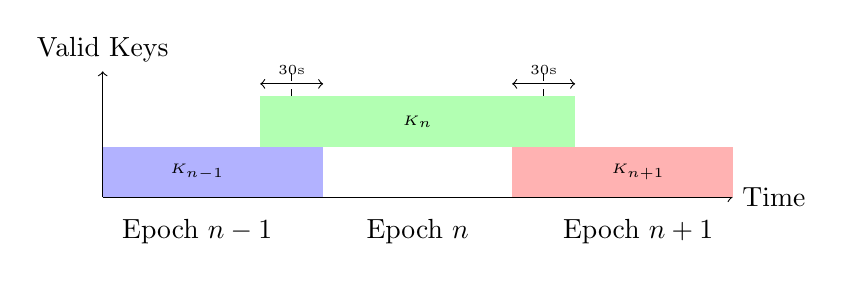
\begin{tikzpicture}[scale=0.8]
    \draw[->] (0,0) -- (10,0) node[right] {Time};
    \draw[->] (0,0) -- (0,2) node[above] {Valid Keys};

    % Epoch boundaries
    \draw[dashed] (3,0) -- (3,2);
    \draw[dashed] (7,0) -- (7,2);

    % Key validity regions
    \fill[blue!30] (0,0) rectangle (3.5,0.8);
    \fill[green!30] (2.5,0.8) rectangle (7.5,1.6);
    \fill[red!30] (6.5,0) rectangle (10,0.8);

    % Labels
    \node at (1.5,0.4) {\tiny $K_{n-1}$};
    \node at (5,1.2) {\tiny $K_n$};
    \node at (8.5,0.4) {\tiny $K_{n+1}$};

    % Grace windows
    \draw[<->] (2.5,1.8) -- (3.5,1.8) node[midway,above] {\tiny 30s};
    \draw[<->] (6.5,1.8) -- (7.5,1.8) node[midway,above] {\tiny 30s};

    % Epoch labels
    \node[below] at (1.5,-0.2) {Epoch $n-1$};
    \node[below] at (5,-0.2) {Epoch $n$};
    \node[below] at (8.5,-0.2) {Epoch $n+1$};
\end{tikzpicture}
\caption{Key validity with grace windows at epoch boundaries}
\end{figure}

\section{Collective Intelligence}

\subsection{Role Distribution}

NanOS implements bio-inspired quorum sensing for role adaptation:

\begin{definition}[Role Set]
$\mathcal{R} = \{\text{Worker}, \text{Explorer}, \text{Sentinel}, \text{Queen}\}$
\end{definition}

\begin{definition}[Target Distribution]
The system maintains:
\begin{equation}
\pi^* = (0.75, 0.125, 0.125, \leq 1/N)
\end{equation}
for (Worker, Explorer, Sentinel, Queen) respectively.
\end{definition}

\subsection{Queen Election Protocol}

\begin{algorithm}[h]
\caption{Deterministic Queen Election}
\begin{algorithmic}[1]
\State \textbf{Trigger:} No queen heartbeat for $T_{\text{absence}} = 10$s
\State $\text{election\_id} \gets \min(\text{visible\_node\_ids})$
\State Broadcast $\langle\text{ELECTION}, \text{election\_id}, \text{my\_id}\rangle$
\State Wait $T_{\text{election}} = 5$s, collect votes
\State $\text{winner} \gets \max(\text{received\_node\_ids})$
\If{$\text{winner} = \text{my\_id}$}
    \State Transition to QUEEN role
    \State Broadcast CORONATION
\EndIf
\end{algorithmic}
\end{algorithm}

\begin{theorem}[Election Convergence]
The election protocol converges in $O(1)$ rounds with probability 1, as the winner is deterministically the highest node ID.
\end{theorem}

\subsection{Gradient Routing}

Distance to queen propagates via gradient descent:
\begin{equation}
d_i = \begin{cases}
0 & \text{if } i = \text{Queen} \\
1 + \min_{j \in \mathcal{N}(i)} d_j & \text{otherwise}
\end{cases}
\end{equation}

where $\mathcal{N}(i)$ is the neighbor set of node $i$.

\subsection{Hebbian Routing (v0.5)}

NanOS v0.5 introduces \textbf{Hebbian routing}: ``Neurons that fire together, wire together.'' Each neighbor connection has a \textit{synaptic weight} $w \in [1, 255]$ that evolves based on communication outcomes.

\begin{definition}[Synaptic Weight Update]
For a communication event with neighbor $j$:
\begin{align}
w_j &\leftarrow \min(255, w_j + 15) & \text{(LTP: success)} \\
w_j &\leftarrow \max(1, w_j - 40) & \text{(LTD: failure)}
\end{align}
\end{definition}

The asymmetric learning rule (reward +15, punishment -40) ensures the network quickly avoids unreliable paths.

\begin{definition}[Neural Routing Cost]
The composite routing cost combines distance and reliability:
\begin{equation}
\text{Cost}(j) = 10 \cdot d_j + \frac{255 - w_j}{8}
\end{equation}
\end{definition}

\begin{theorem}[Reliable Path Selection]
A 2-hop path through a perfect node ($w=255$) has cost $20+0=20$, while a 1-hop path through an unreliable node ($w=1$) has cost $10+31=41$. The network learns to route around bad nodes.
\end{theorem}

\textbf{STDP Bonus}: Fast ACK responses ($<100$ms) receive an additional weight bonus of +5, encouraging low-latency paths.

\subsection{Stigmergia: Digital Pheromones (v0.5)}

Biological ant colonies coordinate through \textbf{stigmergia}: indirect communication via environmental modification. Ants leave chemical trails that evaporate over time, creating dynamic pathways. NanOS v0.5 implements this concept digitally.

\begin{figure}[h]
\centering
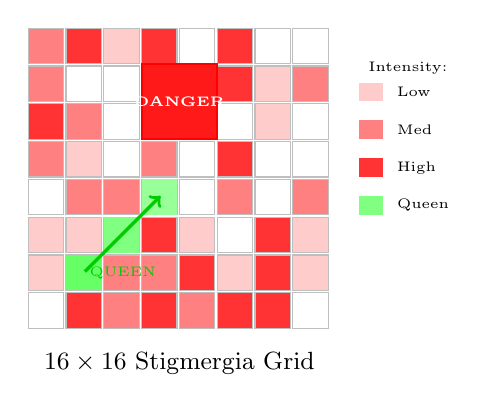
\begin{tikzpicture}[scale=0.6]
    % Grid representation
    \foreach \x in {0,...,7} {
        \foreach \y in {0,...,7} {
            \pgfmathsetmacro{\intensity}{int(random(0,3))}
            \ifnum\intensity=0
                \fill[white] (\x*0.8,\y*0.8) rectangle (\x*0.8+0.75,\y*0.8+0.75);
            \fi
            \ifnum\intensity=1
                \fill[red!20] (\x*0.8,\y*0.8) rectangle (\x*0.8+0.75,\y*0.8+0.75);
            \fi
            \ifnum\intensity=2
                \fill[red!50] (\x*0.8,\y*0.8) rectangle (\x*0.8+0.75,\y*0.8+0.75);
            \fi
            \ifnum\intensity=3
                \fill[red!80] (\x*0.8,\y*0.8) rectangle (\x*0.8+0.75,\y*0.8+0.75);
            \fi
            \draw[gray!50] (\x*0.8,\y*0.8) rectangle (\x*0.8+0.75,\y*0.8+0.75);
        }
    }
    % Danger zone marker
    \fill[red!90] (2.4,4) rectangle (4,5.6);
    \draw[red,thick] (2.4,4) rectangle (4,5.6);
    \node[white,font=\tiny\bfseries] at (3.2,4.8) {DANGER};

    % Queen trail
    \fill[green!60] (0.8,0.8) rectangle (1.55,1.55);
    \fill[green!50] (1.6,1.6) rectangle (2.35,2.35);
    \fill[green!40] (2.4,2.4) rectangle (3.15,3.15);
    \draw[->,green!80!black,very thick] (1.2,1.2) -- (2.8,2.8);
    \node[green!80!black,font=\tiny,below] at (2,1.5) {QUEEN};

    % Labels
    \node[below,font=\small] at (3.2,-0.3) {$16 \times 16$ Stigmergia Grid};

    % Legend
    \node[right,font=\tiny] at (7,5.5) {Intensity:};
    \fill[red!20] (7,4.8) rectangle (7.5,5.2); \node[right,font=\tiny] at (7.6,5) {Low};
    \fill[red!50] (7,4) rectangle (7.5,4.4); \node[right,font=\tiny] at (7.6,4.2) {Med};
    \fill[red!80] (7,3.2) rectangle (7.5,3.6); \node[right,font=\tiny] at (7.6,3.4) {High};
    \fill[green!50] (7,2.4) rectangle (7.5,2.8); \node[right,font=\tiny] at (7.6,2.6) {Queen};
\end{tikzpicture}
\caption{Stigmergia pheromone grid showing danger zones (red) and queen trails (green)}
\label{fig:stigmergia-grid}
\end{figure}

\begin{definition}[Pheromone Types]
NanOS defines four pheromone types stored as 4-bit nibbles:
\begin{align}
\text{DANGER} &= 0 \quad \text{(Jamming, attacks, bad nodes)} \\
\text{QUEEN} &= 1 \quad \text{(Path to queen)} \\
\text{RESOURCE} &= 2 \quad \text{(Objective markers)} \\
\text{AVOID} &= 3 \quad \text{(Suboptimal areas)}
\end{align}
\end{definition}

\begin{definition}[Pheromone Decay]
Pheromone intensity $I \in [0, 15]$ decays over time:
\begin{equation}
I(t + \Delta t) = \max(0, I(t) - 1)
\end{equation}
where $\Delta t = 1$ second. This ensures old information ``evaporates.''
\end{definition}

\begin{figure}[h]
\centering
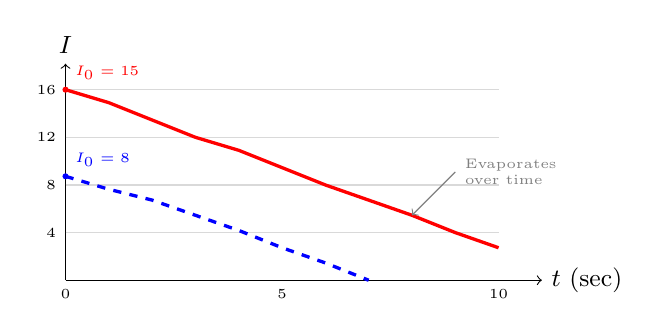
\begin{tikzpicture}[scale=0.55]
    % Axes
    \draw[->] (0,0) -- (11,0) node[right,font=\small] {$t$ (sec)};
    \draw[->] (0,0) -- (0,5) node[above,font=\small] {$I$};

    % Grid
    \foreach \y in {1,...,4} {
        \draw[gray!30] (0,\y*1.1) -- (10,\y*1.1);
        \node[left,font=\tiny] at (0,\y*1.1) {\pgfmathparse{int(\y*4)}\pgfmathresult};
    }

    % Decay curve (starting at 15)
    \draw[red,very thick] (0,4.4) -- (1,4.1) -- (2,3.7) -- (3,3.3) -- (4,3) -- (5,2.6)
                          -- (6,2.2) -- (7,1.85) -- (8,1.5) -- (9,1.1) -- (10,0.75);
    \fill[red] (0,4.4) circle (2pt);
    \node[red,above right,font=\tiny] at (0,4.4) {$I_0=15$};

    % Decay curve (starting at 8)
    \draw[blue,very thick,dashed] (0,2.4) -- (1,2.1) -- (2,1.85) -- (3,1.5)
                                   -- (4,1.15) -- (5,0.75) -- (6,0.4) -- (7,0);
    \fill[blue] (0,2.4) circle (2pt);
    \node[blue,above right,font=\tiny] at (0,2.4) {$I_0=8$};

    % Evaporation annotation
    \draw[<-,gray] (8,1.5) -- (9,2.5) node[right,font=\tiny,align=left] {Evaporates\\over time};

    % Time markers
    \foreach \x in {0,5,10} {
        \node[below,font=\tiny] at (\x,0) {\x};
    }
\end{tikzpicture}
\caption{Pheromone decay: intensity decreases by 1 per second until zero}
\label{fig:pheromone-decay}
\end{figure}

\begin{definition}[Movement Cost Modification]
The terrain movement cost is modified by pheromones:
\begin{equation}
\text{Cost}_{\text{total}} = \text{Cost}_{\text{base}} + 8 \cdot I_{\text{DANGER}} + 4 \cdot I_{\text{AVOID}} - 2 \cdot I_{\text{QUEEN}}
\end{equation}
\end{definition}

\begin{theorem}[Danger Avoidance]
A cell with maximum danger intensity ($I_{\text{DANGER}} = 15$) adds cost $+120$, equivalent to 12 extra distance units. The swarm naturally routes around dangerous zones without explicit coordination.
\end{theorem}

\textbf{Memory Efficiency}: The stigmergia grid uses 2:1 scale mapping ($16 \times 16$ cells covering $32 \times 32$ terrain), with nibble packing requiring only 512 bytes total.

\subsection{Distributed Black Box: ``El Último Aliento'' (v0.5)}

When a node is compromised and terminated, its forensic evidence could be lost. NanOS v0.5 implements a \textbf{distributed black box} where dying nodes transmit their ``last will'' to trusted neighbors.

\begin{figure}[h]
\centering
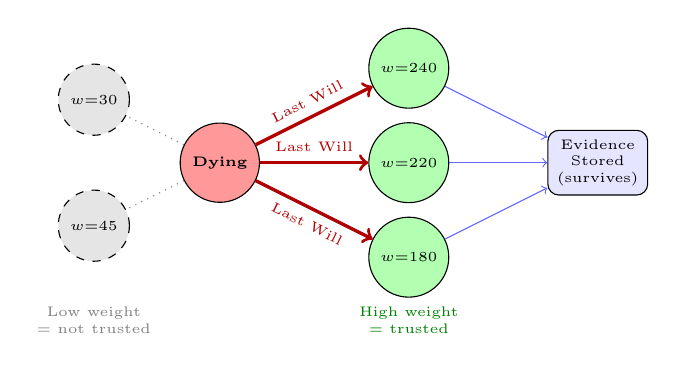
\begin{tikzpicture}[
    node/.style={circle, draw, minimum size=0.8cm, font=\tiny},
    dying/.style={circle, draw, fill=red!40, minimum size=1cm, font=\tiny\bfseries},
    trusted/.style={circle, draw, fill=green!30, minimum size=0.8cm, font=\tiny},
    untrusted/.style={circle, draw, fill=gray!20, dashed, minimum size=0.7cm, font=\tiny},
    scale=0.8
]
    % Dying node
    \node[dying] (d) at (0,0) {Dying};

    % Trusted neighbors (high weight)
    \node[trusted] (t1) at (3,1.5) {$w$=240};
    \node[trusted] (t2) at (3,0) {$w$=220};
    \node[trusted] (t3) at (3,-1.5) {$w$=180};

    % Untrusted neighbors (low weight)
    \node[untrusted] (u1) at (-2,1) {$w$=30};
    \node[untrusted] (u2) at (-2,-1) {$w$=45};

    % Last will arrows (to trusted only)
    \draw[->,very thick,red!70!black] (d) -- node[above,font=\tiny,sloped] {Last Will} (t1);
    \draw[->,very thick,red!70!black] (d) -- node[above,font=\tiny] {Last Will} (t2);
    \draw[->,very thick,red!70!black] (d) -- node[below,font=\tiny,sloped] {Last Will} (t3);

    % No connection to untrusted
    \draw[dotted,gray] (d) -- (u1);
    \draw[dotted,gray] (d) -- (u2);

    % Evidence storage
    \node[draw,rounded corners,fill=blue!10,font=\tiny,align=center] (storage) at (6,0)
        {Evidence\\Stored\\(survives)};
    \draw[->,blue!60] (t1) -- (storage);
    \draw[->,blue!60] (t2) -- (storage);
    \draw[->,blue!60] (t3) -- (storage);

    % Annotation
    \node[font=\tiny,align=center,gray] at (-2,-2.5) {Low weight\\= not trusted};
    \node[font=\tiny,align=center,green!50!black] at (3,-2.5) {High weight\\= trusted};
\end{tikzpicture}
\caption{Distributed Black Box: dying node sends last will to trusted neighbors (selected by Hebbian weight)}
\label{fig:blackbox-flow}
\end{figure}

\begin{definition}[Last Will Testament]
A last will contains:
\begin{itemize}
    \item Node ID and uptime duration
    \item Death reason code (NATURAL, HEAP\_EXHAUSTED, CORRUPTION, ATTACK\_DETECTED, QUEEN\_ORDER, ISOLATION)
    \item Security statistics: bad MAC count, replay attempts, rate limit triggers
    \item Recent security event log (last 8 events)
\end{itemize}
\end{definition}

\begin{definition}[Trusted Recipient Selection]
Last wills are sent to neighbors with highest Hebbian weights:
\begin{equation}
\text{Recipients} = \arg\max_{j \in \mathcal{N}, |\text{Recipients}| \leq 3} w_j
\end{equation}
This ensures forensic data reaches reliable nodes that will preserve and relay it.
\end{definition}

\begin{theorem}[Evidence Survival]
If a node is compromised and forced to suicide, its last will survives in $k$ trusted neighbors. Assuming independent compromise probability $p$ per node, the probability of total evidence loss is $p^k$. With $k=3$ and $p=0.1$, evidence survives with probability $99.9\%$.
\end{theorem}

\textbf{Forensic Query}: Surviving nodes can query the black box by node ID:
\begin{lstlisting}[language=C]
int blackbox_query_death(uint32_t node_id,
    uint8_t *death_reason, uint16_t *bad_mac_count,
    uint8_t *uptime_hours);
\end{lstlisting}

\subsection{Artificial Immune System (AIS) (v0.6)}

The biological immune system does not require prior knowledge of pathogens---it simply recognizes ``non-self'' patterns. NanOS v0.6 implements the \textbf{Negative Selection Algorithm} for 0-day anomaly detection.

\begin{definition}[Detector]
A detector $d = (p, m)$ consists of a pattern $p \in \{0,1\}^{64}$ and mask $m \in \{0,1\}^{64}$. A detector matches antigen $a$ if:
\begin{equation}
\text{affinity}(d, a) = \max_{i}\{j : p[i:i+j] \oplus a[i:i+j] = 0\} \geq \theta
\end{equation}
where $\theta = 6$ bits (r-contiguous matching threshold).
\end{definition}

\begin{definition}[Negative Selection]
During the \textbf{thymus phase} (5 seconds at boot), detectors are generated randomly and tested against ``self'' samples. Detectors that match self are eliminated (anergy), ensuring mature detectors only recognize ``non-self.''
\begin{equation}
D_{\text{mature}} = \{d \in D_{\text{generated}} : \forall s \in S_{\text{self}}, \text{affinity}(d, s) < \theta\}
\end{equation}
\end{definition}

\begin{theorem}[0-Day Detection]
Unlike signature-based systems, AIS detects anomalies without prior attack knowledge. Any traffic pattern that does not match the learned ``self'' profile triggers an alert. This enables detection of previously unknown attacks (0-days).
\end{theorem}

\begin{figure}[h]
\centering
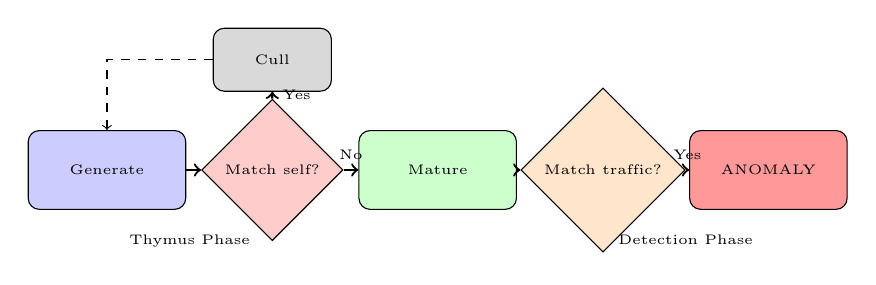
\begin{tikzpicture}[scale=0.7]
    % Thymus phase
    \node[draw, rounded corners, fill=blue!20, minimum width=2cm, minimum height=1cm] (gen) at (0,0) {\tiny Generate};
    \node[draw, diamond, fill=red!20, minimum width=1.5cm] (check) at (3,0) {\tiny Match self?};
    \node[draw, rounded corners, fill=gray!30, minimum width=1.5cm, minimum height=0.8cm] (cull) at (3,2) {\tiny Cull};
    \node[draw, rounded corners, fill=green!20, minimum width=2cm, minimum height=1cm] (mature) at (6,0) {\tiny Mature};

    % Detection phase
    \node[draw, diamond, fill=orange!20, minimum width=1.5cm] (detect) at (9,0) {\tiny Match traffic?};
    \node[draw, rounded corners, fill=red!40, minimum width=2cm, minimum height=1cm] (alert) at (12,0) {\tiny ANOMALY};

    % Arrows
    \draw[->, thick] (gen) -- (check);
    \draw[->, thick] (check) -- node[right, font=\tiny] {Yes} (cull);
    \draw[->, thick] (check) -- node[above, font=\tiny] {No} (mature);
    \draw[->, thick] (mature) -- (detect);
    \draw[->, thick] (detect) -- node[above, font=\tiny] {Yes} (alert);
    \draw[->, dashed] (cull) -| (gen);

    % Labels
    \node[font=\tiny, below] at (1.5, -1) {Thymus Phase};
    \node[font=\tiny, below] at (10.5, -1) {Detection Phase};
\end{tikzpicture}
\caption{AIS Negative Selection: detectors that match ``self'' are eliminated}
\label{fig:ais-negative-selection}
\end{figure}

\textbf{Integration}: When AIS detects an anomaly, it triggers a coordinated response:
\begin{itemize}
    \item \textbf{Stigmergia}: Emits DANGER pheromone at current location
    \item \textbf{Black Box}: Records EVENT\_AIS\_ANOMALY\_ALERT
    \item \textbf{Hebbian}: Applies LTD (depression) to source node's weight
    \item \textbf{Broadcast}: Sends ALARM pheromone to swarm
\end{itemize}

\subsection{Code Polymorphism: ``El Camaleón'' (v0.6)}

Traditional exploits can be replayed against any node running identical binaries.
NanOS v0.6 introduces \textbf{Code Polymorphism} to ensure each node has a unique
binary fingerprint, making mass exploitation infeasible.

\textbf{ASLR} (Address Space Layout Randomization):
\begin{itemize}
    \item Stack base: 8 bits of entropy (256 possible bases)
    \item Heap base: 6 bits of entropy (64 possible bases)
    \item Combined: $2^{14} = 16,384$ layout combinations per node
\end{itemize}

\textbf{Stack Canaries}: Random 32-bit values placed on stack to detect buffer overflows.
Canary violations trigger immediate security response (Black Box event + apoptosis).

\textbf{Binary Signatures}: Each node generates a unique 128-bit fingerprint derived from:
\[
\text{Signature} = H(\text{node\_id} \| \text{RNG\_seed} \| \text{boot\_tick} \| \text{ASLR\_entropy})
\]

\textbf{Timing Jitter}: Random delays of $[10, 100]\mu s$ applied to cryptographic operations
to mitigate timing side-channel attacks.

\begin{figure}[h]
\centering
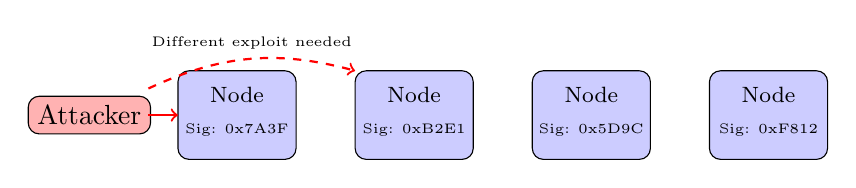
\begin{tikzpicture}[scale=0.75]
    % Node boxes with different fingerprints
    \foreach \i/\sig in {0/0x7A3F, 3/0xB2E1, 6/0x5D9C, 9/0xF812} {
        \draw[fill=blue!20, rounded corners] (\i, 0) rectangle (\i+2, 1.5);
        \node at (\i+1, 1.1) {\footnotesize Node};
        \node[font=\tiny] at (\i+1, 0.5) {Sig: \sig};
    }

    % Attacker
    \node[draw, fill=red!30, rounded corners] at (-1.5, 0.75) {Attacker};

    % Exploit arrows
    \draw[->, thick, red] (-0.5, 0.75) -- (0, 0.75);
    \draw[->, thick, red, dashed] (-0.5, 1.2) to[bend left=20] (3, 1.5);
    \node[font=\tiny, above] at (1.25, 1.7) {Different exploit needed};
\end{tikzpicture}
\caption{Code Polymorphism: each node requires a unique exploit}
\label{fig:code-polymorphism}
\end{figure}

\textbf{Diversity Score}: Quantifies uniqueness ($0$--$255$, higher = more diverse):
\[
\text{Score} = \text{popcount}(\text{stack\_offset}) \cdot 8 + \text{popcount}(\text{heap\_offset}) \cdot 8 + \sum_{i=0}^{15} \text{popcount}(\text{sig}[i])
\]

\subsection{Hardware Validation: ``El Centinela del Silicio'' (v0.6)}

Software can be fooled, but tortured hardware reveals the truth. NanOS v0.6 implements
\textbf{Hardware Validation} to detect physical manipulation, sensor tampering, and fault injection attacks.

\textbf{Sensor Monitoring}: Continuous validation of physical parameters:
\begin{itemize}
    \item Temperature: $[-40, 85]$°C operating range, max $\Delta T = 10$°C/s
    \item Voltage: $[2.7, 3.6]$V operating range, glitch detection at $\Delta V > 100$mV
    \item Clock: 5\% drift tolerance, 3 consecutive glitches trigger alarm
\end{itemize}

\textbf{Memory Canaries}: Random values placed at critical locations:
\begin{equation}
\text{Canary}_i = \texttt{0xC0DEBABE} \oplus \text{address}_i
\end{equation}
If $\text{Canary}_i^{\text{current}} \neq \text{Canary}_i^{\text{expected}}$, memory corruption is detected.

\textbf{Flash CRC}: Registered code blocks are verified periodically:
\begin{equation}
\text{Valid} = \text{CRC32}(\text{flash}[a:a+s]) = \text{CRC32}_{\text{baseline}}
\end{equation}

\textbf{Trust Score}: Hardware trustworthiness quantified as:
\begin{equation}
\text{TrustScore} = 255 - \text{AnomalyScore} - 10 \cdot |\text{Violations}|
\end{equation}

\textbf{Defense in Depth}: Hardware Validation complements other security layers:
\begin{itemize}
    \item AIS detects network anomalies
    \item Polymorphism makes binaries unique
    \item Hardware Validation detects physical attacks
\end{itemize}
An attacker must defeat all layers to compromise a node.

\subsection{Genetic Tuning: Evolutionary Parameter Optimization (v0.7)}

NanOS v0.7 introduces \textbf{Genetic Tuning}, enabling the Queen to automatically
optimize NERT protocol parameters using genetic algorithms. The system maintains
a population of \textbf{genomes}---32-byte structures encoding timing, gossip, and
security parameters---and distributes them to sub-swarms for evaluation.

\begin{definition}[Genome Structure]
A genome $G$ encodes $n=15$ parameters as genes:
\begin{equation}
G = \{g_1, g_2, \ldots, g_{15}\} \text{ where } g_i \in [L_i, U_i]
\end{equation}
with bounded ranges ensuring valid configurations.
\end{definition}

\textbf{Fitness Function}: The fitness of each genome combines five metrics:
\begin{equation}
F(G) = 0.30 \cdot T + 0.20 \cdot L + 0.25 \cdot R + 0.15 \cdot S + 0.10 \cdot V
\end{equation}
where $T$ = throughput, $L$ = inverse latency, $R$ = reliability, $S$ = security (inverse violations), $V$ = survival (uptime + neighbors).

\textbf{Genetic Operators}:
\begin{itemize}
    \item \textbf{Tournament Selection}: $k=3$ random genomes compete, highest fitness advances
    \item \textbf{Two-Point Crossover}: Parents exchange gene segments between two random points
    \item \textbf{Bounded Mutation}: 5\% probability per gene, constrained to valid ranges
    \item \textbf{Elitism}: Top 10\% genomes preserved unchanged across generations
\end{itemize}

\textbf{Protocol Messages}:
\begin{itemize}
    \item \texttt{CONFIG\_UPDATE (0x14)}: Queen distributes genome to sub-swarm (authenticated)
    \item \texttt{TELEMETRY\_REPORT (0x15)}: Workers report metrics to Queen (periodic)
\end{itemize}

\subsection{Judas Nodes: Active Honeypots (v0.7)}

\textbf{Judas Nodes} are Workers that, upon detecting intrusion, feign vulnerability
to capture attacker payloads before self-destructing. This transforms compromised
nodes into threat intelligence sources.

\begin{definition}[Judas State Machine]
A Judas node transitions through states:
\begin{equation}
\text{DORMANT} \xrightarrow{\text{trigger}} \text{SUSPICIOUS} \xrightarrow{\text{threshold}} \text{ENGAGING} \xrightarrow{\text{payload}} \text{CAPTURING} \xrightarrow{\text{complete}} \text{DETONATING}
\end{equation}
\end{definition}

\textbf{Activation Triggers}: Bad MACs ($\geq 3$), replay attempts ($\geq 2$), anomalous probes ($\geq 5$).

\textbf{Protocol Messages}:
\begin{itemize}
    \item \texttt{JUDAS\_ENGAGE (0x16)}: Notifies Queen of attacker engagement
    \item \texttt{JUDAS\_CAPTURE (0x17)}: Transmits captured attacker payload
    \item \texttt{JUDAS\_FORENSICS (0x18)}: Complete BlackBox before apoptosis
\end{itemize}

\begin{theorem}[Forensic Survival]
If a Judas node captures payload $P$ and transmits to $k$ trusted neighbors before detonation,
evidence survives with probability $1 - p^k$ where $p$ is single-node compromise probability.
With $k=3$ and $p=0.1$, survival probability exceeds $99.9\%$.
\end{theorem}

\subsection{Covert Channels: Physical Side-Channels (v0.7)}

For air-gapped environments, NanOS v0.7 implements \textbf{Covert Channels} using
physical side-channels: optical (LED/light sensor) and acoustic (buzzer/microphone).

\textbf{Optical Channel}:
\begin{itemize}
    \item Transmitter: LED controlled via PWM
    \item Receiver: Photoresistor/photodiode on ADC
    \item Modulation: Manchester encoding (self-clocking)
    \item Data rate: 10--100 bps
\end{itemize}

\textbf{Acoustic Channel}:
\begin{itemize}
    \item Transmitter: Piezoelectric buzzer with PWM
    \item Receiver: Analog microphone or I2S
    \item Modulation: FSK (1kHz/2kHz audible or 18kHz/20kHz ultrasonic)
    \item Data rate: 50--200 bps
\end{itemize}

\begin{definition}[Manchester Encoding]
Each bit $b$ is encoded as a transition at mid-period:
\begin{equation}
\text{encode}(b) = \begin{cases}
\text{HIGH} \to \text{LOW} & \text{if } b = 0 \\
\text{LOW} \to \text{HIGH} & \text{if } b = 1
\end{cases}
\end{equation}
Transitions provide clock recovery without separate synchronization.
\end{definition}

\textbf{Security}: Covert channel data is encrypted with the same ChaCha8 session key
and includes sequence numbers for anti-replay protection. Maximum payload is 16 bytes per frame.

\section{Engineering Implementation}

\subsection{Memory Layout (ARM Cortex-M3)}

\begin{lstlisting}[language=C, caption=Memory configuration]
#define NERT_COMPACT_MODE       1
#define NERT_HEADER_SIZE        12  // bytes
#define NERT_MAX_PAYLOAD        64  // bytes
#define NERT_MAX_CONNECTIONS    4
#define NERT_WINDOW_SIZE        2
#define NERT_DEDUP_CACHE_SIZE   8
#define BLOOM_BYTES             32
#define GOSSIP_CACHE_SIZE       32
\end{lstlisting}

\subsection{CPU Cycle Budget}

\begin{table}[h]
\centering
\small
\begin{tabular}{lr}
\toprule
\textbf{Operation} & \textbf{Cycles (Cortex-M3)} \\
\midrule
ChaCha8 encrypt (32B) & $\sim$2,000 \\
Poly1305 MAC & $\sim$1,500 \\
FEC encode (4$\to$6) & $\sim$500 \\
FEC decode (6$\to$4) & $\sim$1,000 \\
Header parse & $\sim$100 \\
Bloom filter check & $\sim$50 \\
\midrule
\textbf{Total per packet} & $\sim$5,000 \\
\bottomrule
\end{tabular}
\caption{Computational cost per packet}
\end{table}

At 48 MHz, this yields a theoretical throughput of 9,600 packets/second.

\subsection{Supported Platforms}

\begin{itemize}
    \item \textbf{x86}: QEMU with e1000 NIC, Multiboot2 boot
    \item \textbf{ARM Cortex-M3}: QEMU LM3S, real hardware (STM32)
    \item \textbf{ARM64}: QEMU virt, Raspberry Pi 4
    \item \textbf{ESP32}: ESP-IDF and PlatformIO, WiFi/LoRa
    \item \textbf{ESP8266}: Ultra-lightweight variant
\end{itemize}

\section{Security Evaluation}

\subsection{Threat Model}

We assume a Dolev-Yao adversary who can:
\begin{itemize}
    \item Intercept all network traffic
    \item Inject arbitrary packets
    \item Replay captured packets
    \item Perform denial-of-service attacks
\end{itemize}

The adversary does \textbf{not} have access to the master key $K_m$.

\subsection{Experimental Results}

\begin{table}[h]
\centering
\small
\begin{tabular}{lrr}
\toprule
\textbf{Attack Type} & \textbf{Packets Sent} & \textbf{Rejected} \\
\midrule
Replay & 5 & 5 (100\%) \\
Fuzzing & 15 & 15 (100\%) \\
Fake Queen & 5 & 5 (100\%) \\
DoS (250 pkt) & 250 & 250 (100\%) \\
\midrule
\textbf{Total} & 275 & 275 (100\%) \\
\bottomrule
\end{tabular}
\caption{Attack rejection rates (test suite)}
\end{table}

Under intensive manual attack (1,191 malicious packets):
\begin{equation}
\text{Rejection Rate} = \frac{1191}{1206} = 98.76\%
\end{equation}

The 1.24\% accepted packets were legitimate inter-node traffic.

\subsection{Security Properties}

\begin{property}[Confidentiality]
All payloads are encrypted with ChaCha8. Without $K_m$, ciphertext is indistinguishable from random.
\end{property}

\begin{property}[Integrity]
Poly1305 MAC detects any modification with probability $1 - 2^{-64}$.
\end{property}

\begin{property}[Authenticity]
Only nodes possessing $K_m$ can generate valid MACs.
\end{property}

\begin{property}[Replay Resistance]
Nonce = (node\_id, counter, timestamp) ensures uniqueness. The 64-bit replay window bitmap catches duplicates within $\pm 32$ sequence numbers.
\end{property}

\section{Related Work}

\textbf{Swarm Protocols}: Kilobot \cite{rubenstein2012kilobot} uses infrared for local communication but lacks encryption. E-puck \cite{mondada2009puck} relies on Bluetooth with standard security.

\textbf{Lightweight Crypto}: PRESENT \cite{bogdanov2007present} and SIMON/SPECK \cite{beaulieu2015simon} target ultra-constrained devices but require block cipher modes. ChaCha8 provides native stream cipher operation.

\textbf{Gossip Protocols}: Epidemic routing \cite{vahdat2000epidemic} and SWIM \cite{das2002swim} inspire our probabilistic relay, enhanced with cryptographic authentication.

\section{Conclusion}

NanOS with NERT demonstrates that secure, reliable swarm communication is achievable within 24KB RAM. The key innovations are:

\begin{enumerate}
    \item \textbf{Adaptive reliability}: Four classes from fire-forget to FEC+multipath
    \item \textbf{Lightweight crypto}: ChaCha8+Poly1305 with 64-bit MACs
    \item \textbf{Clock-drift tolerance}: Grace window key rotation
    \item \textbf{Bio-inspired coordination}: Quorum sensing and gradient routing
    \item \textbf{Hebbian routing (v0.5)}: Neural-inspired path learning with LTP/LTD asymmetric updates
    \item \textbf{DoS resilience (v0.5)}: Per-node rate limiting and behavioral reputation system
    \item \textbf{Stigmergia (v0.5)}: Digital pheromones with temporal decay for emergent spatial coordination
    \item \textbf{Distributed Black Box (v0.5)}: ``Last Will'' forensic evidence that survives node death
    \item \textbf{Artificial Immune System (v0.6)}: Negative Selection for 0-day anomaly detection without signatures
    \item \textbf{Code Polymorphism (v0.6)}: ``El Camaleón'' --- binary diversity preventing exploit reuse across nodes
    \item \textbf{Hardware Validation (v0.6)}: ``El Centinela del Silicio'' --- physical layer security through sensor monitoring and fault detection
    \item \textbf{Genetic Tuning (v0.7)}: Evolutionary auto-optimization of NERT parameters using genetic algorithms with fitness-based selection
    \item \textbf{Judas Nodes (v0.7)}: Active honeypots that capture attacker payloads before self-destructing, generating threat intelligence
    \item \textbf{Covert Channels (v0.7)}: Physical side-channels (optical/acoustic) enabling air-gap communication via LED and buzzer modulation
\end{enumerate}

Version 0.5 introduces a ``distributed brain'' where the swarm learns from experience: successful communications strengthen synaptic weights while failures cause severe depression, enabling automatic route optimization without central coordination. The stigmergia system adds spatial memory through evaporating pheromones, while the black box ensures forensic evidence survives even when nodes are compromised and terminated.

Version 0.6 adds an \textbf{Artificial Immune System} (AIS) based on the Negative Selection algorithm. Unlike signature-based intrusion detection, AIS learns what ``normal'' traffic looks like and flags anything that deviates---enabling detection of previously unknown attacks (0-days). The system integrates with all previous mechanisms: detected anomalies trigger DANGER pheromones (stigmergia), are recorded for forensics (black box), and penalize the source node's reputation (Hebbian).

Version 0.6 also introduces \textbf{Code Polymorphism} (``El Camaleón''), ensuring each node has a unique binary fingerprint. Through ASLR (stack and heap randomization), stack canaries, 128-bit binary signatures, and timing jitter, exploits developed for one node cannot be replayed against others. With $2^{14}$ ASLR combinations per node, compromising a 1000-node swarm requires developing 1000 unique exploits---fundamentally changing the economics of attack.

Finally, v0.6 introduces \textbf{Hardware Validation} (``El Centinela del Silicio''), providing physical layer security through continuous monitoring of temperature, voltage, and clock frequency. Memory canaries detect unauthorized modifications, while flash CRC verification catches firmware tampering. The system computes a hardware ``Trust Score'' that other security layers can use to assess node reliability. This completes a defense-in-depth architecture where attackers must simultaneously defeat network-level (AIS), binary-level (Polymorphism), and physical-level (Hardware Validation) protections.

Version 0.7 introduces three evolutionary capabilities. \textbf{Genetic Tuning} enables the Queen to automatically optimize NERT parameters using genetic algorithms---tournament selection, two-point crossover, and bounded mutation evolve a population of genomes distributed to sub-swarms for A/B testing. Fitness evaluation combines throughput (30\%), latency (20\%), reliability (25\%), security (15\%), and survival (10\%) metrics. \textbf{Judas Nodes} transform compromised nodes into threat intelligence sources: upon detecting intrusion, they feign vulnerability to capture attacker payloads before detonating, transmitting forensic evidence via JUDAS\_FORENSICS pheromones. This turns every attempted compromise into intelligence gathering. \textbf{Covert Channels} enable communication in air-gapped environments through physical side-channels---optical (LED/light sensor with Manchester encoding at 10-100 bps) and acoustic (buzzer/microphone with FSK modulation at 50-200 bps). All covert traffic is encrypted with the same ChaCha8 session key, maintaining end-to-end security even across physical media.

Future work includes formal verification of the protocol state machine and evaluation on physical swarm hardware.

\section*{Acknowledgments}

This work was developed as part of the NanOS open-source project.

\begin{thebibliography}{9}
\bibitem{bernstein2008chacha}
D.J. Bernstein, ``ChaCha, a variant of Salsa20,'' SASC 2008.

\bibitem{rubenstein2012kilobot}
M. Rubenstein et al., ``Kilobot: A low cost scalable robot system for collective behaviors,'' ICRA 2012.

\bibitem{mondada2009puck}
F. Mondada et al., ``The e-puck, a robot designed for education in engineering,'' 2009.

\bibitem{bogdanov2007present}
A. Bogdanov et al., ``PRESENT: An ultra-lightweight block cipher,'' CHES 2007.

\bibitem{beaulieu2015simon}
R. Beaulieu et al., ``The SIMON and SPECK families of lightweight block ciphers,'' DAC 2015.

\bibitem{vahdat2000epidemic}
A. Vahdat and D. Becker, ``Epidemic routing for partially-connected ad hoc networks,'' Duke Tech Report, 2000.

\bibitem{das2002swim}
A. Das et al., ``SWIM: Scalable weakly-consistent infection-style process group membership protocol,'' DSN 2002.
\end{thebibliography}

\appendix

\section{Nonce Construction}

\begin{lstlisting}[language=C]
void build_nonce(uint8_t nonce[12],
                 uint16_t node_id,
                 uint32_t counter,
                 uint32_t timestamp) {
    nonce[0] = node_id & 0xFF;
    nonce[1] = node_id >> 8;
    nonce[2] = 0; // reserved
    nonce[3] = 0;
    memcpy(&nonce[4], &counter, 4);
    memcpy(&nonce[8], &timestamp, 4);
}
\end{lstlisting}

\section{Bloom Filter Hash Functions}

\begin{lstlisting}[language=C]
uint8_t bloom_hash0(uint16_t node, uint16_t seq, uint8_t type) {
    return (node * 31 + seq * 0x85EBCA6B + type * 0xC2B2AE35) % 256;
}

uint8_t bloom_hash1(uint16_t node, uint16_t seq, uint8_t type) {
    return (seq * 31 + node * 0xCC9E2D51 + type * 0x1B873593) % 256;
}

uint8_t bloom_hash2(uint16_t node, uint16_t seq, uint8_t type) {
    uint32_t h = (type | (seq << 8)) ^ node;
    h ^= h >> 16; h *= 0x85EBCA6B;
    h ^= h >> 13; h *= 0xC2B2AE35;
    return (h ^ (h >> 16)) % 256;
}
\end{lstlisting}

\end{document}
